\documentclass[a4paper, oneside, 12pt, english]{article}
\usepackage{geometry}
\geometry{
	a4paper,
	total={154mm,232mm},
	left=28mm,
	top=32mm,
}
\setlength{\parskip}{0.85em}
\setlength{\parindent}{2.6em}
\usepackage{array}
\usepackage{amsmath}
\usepackage{amssymb}
\usepackage{amsfonts} 
\usepackage{enumerate}
\usepackage{graphicx}
\usepackage{url}
\usepackage{color}
\usepackage{wrapfig}
\usepackage{systeme}
\usepackage{tabularx}
\usepackage{subfig}
\usepackage{hyperref}
\usepackage[authoryear, round]{natbib}
\usepackage[dvipsnames]{xcolor}
\usepackage{booktabs}
\usepackage{multirow}


\newcommand{\rw}{\color{red}\textbf{?} \color{black}}		% When something needs to be reworded

\begin{document}
\begin{titlepage}
	\newcommand{\HRule}{\rule{\linewidth}{0.5mm}}
	\center
	\textsc{\LARGE Université de Liège}\\[1cm]
	\textsc{\Large Faculté des Sciences Appliquées}\\[2cm]
		
	\HRule \\[0.5cm]
	{ \huge \bfseries Real-time Voice Cloning}\\[0.2cm]
	\HRule \\[2cm]

	\begin{minipage}{0.4\textwidth}
		\begin{flushleft} \Large
			\emph{Author:}\\
			Corentin \textsc{Jemine}
		\end{flushleft}
	\end{minipage}
	~
	\begin{minipage}{0.4\textwidth}
		\begin{flushright} \Large
			\emph{Supervisor:} \\
			Prof. Gilles \textsc{Louppe}
		\end{flushright}
	\end{minipage}\\[4cm]
	
	{\LARGE Academic year 2018 - 2019}\\[1cm]
	
	
\includegraphics{images/uliege_logo.jpg}\\[1.25cm]
	
	\textit{Graduation studies conducted for obtaining the Master's degree \\in Data Science by Corentin Jemine}
	
	\vfill
\end{titlepage}
\setcounter{page}{2}

\section*{Abstract}
Recent advances in deep learning have shown impressive results in the domain of text-to-speech. To this end, a deep neural network is usually trained using a corpus of several hours of professionally recorded speech from a single speaker. Giving a new voice to such a model is highly expensive, as it requires recording a new dataset and retraining the model. A recent research introduced a three-stage pipeline that allows to clone a voice unseen during training from only a few seconds of reference speech, and without retraining the model. The authors share remarkably natural-sounding results, but provide no implementation. We reproduce this framework and open-source the first public implementation of it. We adapt the framework with a newer vocoder model, so as to make it run in real-time.
\clearpage

\tableofcontents
\clearpage

\section{Introduction}
% What is now possible with deep learning in TTS
Deep learning models have become predominant in many fields of applied machine learning. text-to-speech (TTS), the process of synthesizing artificial speech from a text prompt, is no exception. Deep models that would produce more natural-sounding speech than the traditional concatenative approaches begun appearing in 2016. Much of the research focus has been since gathered around making these deep models more efficient, more natural, or training them in an end-to-end fashion. Inference has come from being hundreds of times slower than real-time on GPU \citep{WaveNet} to possible in real-time on a mobile CPU \citep{WaveRNN}. As for the quality of the generated speech, \citet{Tacotron2} demonstrate near human naturalness. Interestingly, speech naturalness is best rated with subjective metrics; and comparison with actual human speech leads to the conclusion that there might be such a thing as "speech more natural than human speech". In fact, some argue that the human naturalness threshold has already been crossed \citep{MOSNaturalness}.

% The state of things in TTS
Datasets of professionally recorded speech are a scarce resource. Synthesizing a natural voice with a correct pronunciation, lively intonation and a minimum of background noise requires training data with the same qualities. Furthermore, data efficiency often remains one of the shortcomings of deep learning. Training a common text-to-speech model such as Tacotron \citep{Tacotron1} typically requires tens of hours of speech. Yet the ability of generating speech with any voice is attractive for a range of applications be they useful or merely a matter of customization. Research has led to frameworks for voice conversion and voice cloning. They differ in that voice conversion is a form of style transfer on a speech segment from a voice to another, whereas voice cloning consists in capturing the voice of a speaker to perform text-to-speech on arbitrary inputs. 

% What voice cloning is about
While the complete training of a single-speaker TTS model is technically a form of voice cloning, the interest rather lies in creating a fixed model that is able to incorporate newer voices with little data. The common approach is to condition a TTS model trained to generalize to new speakers on an embedding of the voice to clone~\citep{DeepVoice2, CloningFewSamples, SV2TTS}. The embedding is low-dimensional and derived by a speaker encoder model that takes reference speech as input. This approach is typically more data efficient than training a separate TTS model for each speaker, in addition to being orders of magnitude faster and less computationally expensive. Interestingly, there is a large discrepancy between the duration of reference speech needed to clone a voice among the different methods, ranging from half an hour per speaker to only a few seconds. This factor is usually determining of the similarity of the generated voice with respect to the true voice of the speaker.

% What we want to achieve
Our objective is to achieve a powerful form of voice cloning. The resulting framework must be able to operate in a zero-shot setting, that is, for speakers unseen during training. It should incorporate a speaker's voice with only a few seconds of reference speech. These desired results are shown to be fulfilled by \citep{SV2TTS}. Their results are impressive\footnote{\url{https://google.github.io/tacotron/publications/speaker_adaptation/index.html}}, but not backed by any public implementation. We reproduce their framework and make our implementation open-source\footnote{\color{red} repo link}. In addition, we integrate a model based on \citep{WaveRNN} in the framework to make it run in real-time, i.e. to generate speech in a time shorter or equal to the duration of the produced speech. \color{red} add a word about our results \color{black}

% Structure of the thesis
The structure of this document goes as follows. We begin with a short introduction on TTS methods that involve machine learning. Follows a review of the evolution of the state of the art for TTS and for voice cloning. We then present the work of \citep{SV2TTS} along with our own implementation. We conclude with a presentation of a toolbox we designed to interface the framework.


\section{A review of text-to-speech methods in machine learning}
\subsection{Statistical parametric speech synthesis}
% The SPSS pipeline
Statistical parametric speech synthesis (SPSS) refers to a group of data-driven TTS methods that emerged in the late 90s. In SPSS, the relationship between the features computed on the input text and the output acoustic features is learned by a statistical generative model (called the acoustic model). A complete SPSS framework thus also includes a pipeline to extract features from the text to synthesize, as well as a system able to reconstruct an audio waveform from the acoustic features produced by the acoustic model (such a system is called a vocoder). Unlike the acoustic model, these two parts of the framework may be entirely engineered and make use of no statistical methods. While modern deep TTS models are usually not referred to as SPSS, the SPSS pipeline as depicted in figure \ref{spss_framework} applies just as well to those newer methods.

\begin{figure}[h]
	\centering
	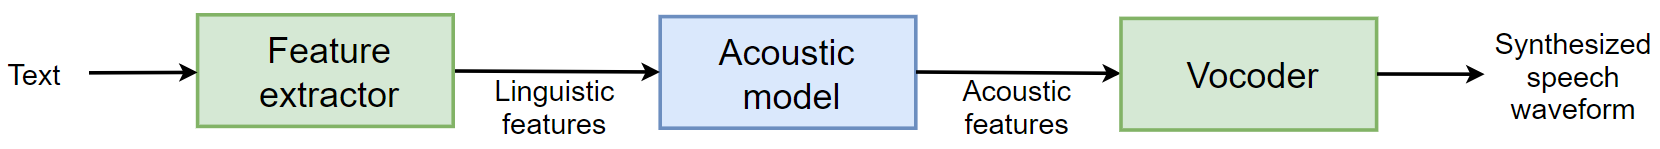
\includegraphics[width=\linewidth]{images/spss_framework.png}
	\caption{The general SPSS pipeline. The blue box is purely a statistical model while the green boxes can be engineered processes or/and statistical models.}
	\label{spss_framework}
\end{figure}

% Purpose of the feature extractor
The role of the feature extractor is to provide data that is more indicative of what the speech produced by the model is expected to sound like. Speech is a complex process, and directly feeding characters to a weak acoustic model will prove not to be effective. Providing additional features from natural language processing (NLP) techniques may greatly reduce the extent of the task to be learned by the acoustic model. It may however result in trade-offs when it comes to naturalness, especially for rare or unknown words. Indeed, manually engineered heuristics do not quite fully characterize all intricacies of spoken language. For this reason, feature extraction can also be done with trained models. The line between the feature extractor and the acoustic model can then become blurry, especially for deep models. In fact, a tendency that is common across all areas where deep models have overtaken traditional machine learning techniques is for feature extraction to consist of less heuristics, as highly nonlinear models become able to operate at higher levels of abstraction.

% Feature extraction techniques
A common feature extraction technique is to build frames that will integrate surrounding context in a hierarchical fashion. For example, a frame at the syllable level could include the word that comprises it, its position in the word, the neighbouring syllables, the phonemes that make up the syllable, ... The lexical stress and accent of individual syllables can be predicted by a statistical model such as a decision tree. To encode prosody, a set of rules such as ToBI \citep{TOBI} can be used. Ultimately, there remains a work of feature engineering to present a frame as a numerical object to the model, e.g. categorical features are typically encoded using a one-hot representation.

% Spectrogram vs waveform
The reason why the acoustic model does not directly predict an audio waveform is that audio happens to be difficult to model: it is a particularly dense domain and audio signals are typically highly nonlinear. A representation that brings out features in a more tractable manner is the time-frequency domain. Spectrograms are smoother and much less dense than their waveform counterpart. They also have the benefit of being two-dimensional, thus allowing models to better leverage spatial connectivity. Unfortunately, a spectrogram is a lossy representation of the waveform that discards the phase. There is no unique inverse transformation function, and deriving one that produces natural-sounding results is not trivial. When referring to speech, this generative function is called a vocoder. The choice of the vocoder is an important factor in determining the quality of the generated audio.

% Evaluation metrics


\subsection{Evolution of the state of the art in text-to-speech}
The state of the art in SPSS has for long remained a hidden Markov model (HMM) based framework \citep{Tokuda-2013}. This approach, laid out in figure \ref{hmm_spss_framework}, consists in clustering the linguistic features extracted from the input text with a decision tree, and to train a HMM per cluster \citep{HMMTTS}. The HMMs are tasked to produce a distribution over spectrogram coefficients, their derivative, second derivative and a binary flag that indicates which parts of the generated audio should contain voice. With the maximum likelihood parameter generation algorithm (MLPG) \citep{Tokuda-2000}, spectrogram coefficients are sampled from this distribution and eventually fed to the MLSA vocoder \citep{MLSA}. It is possible to modify the voice generated by conditioning the HMMs on a speaker or tuning the generated speech parameters with adaptation or interpolation techniques \citep{HMMSpeakerInterpolation}. Note that, while this framework used to be state of the art for SPSS, it was still inferior in terms of the naturalness of the generated speech compared to the well-established concatenative approaches.

\begin{figure}[h]
	\centering
	\begin{minipage}{.45\linewidth}
		\centering
		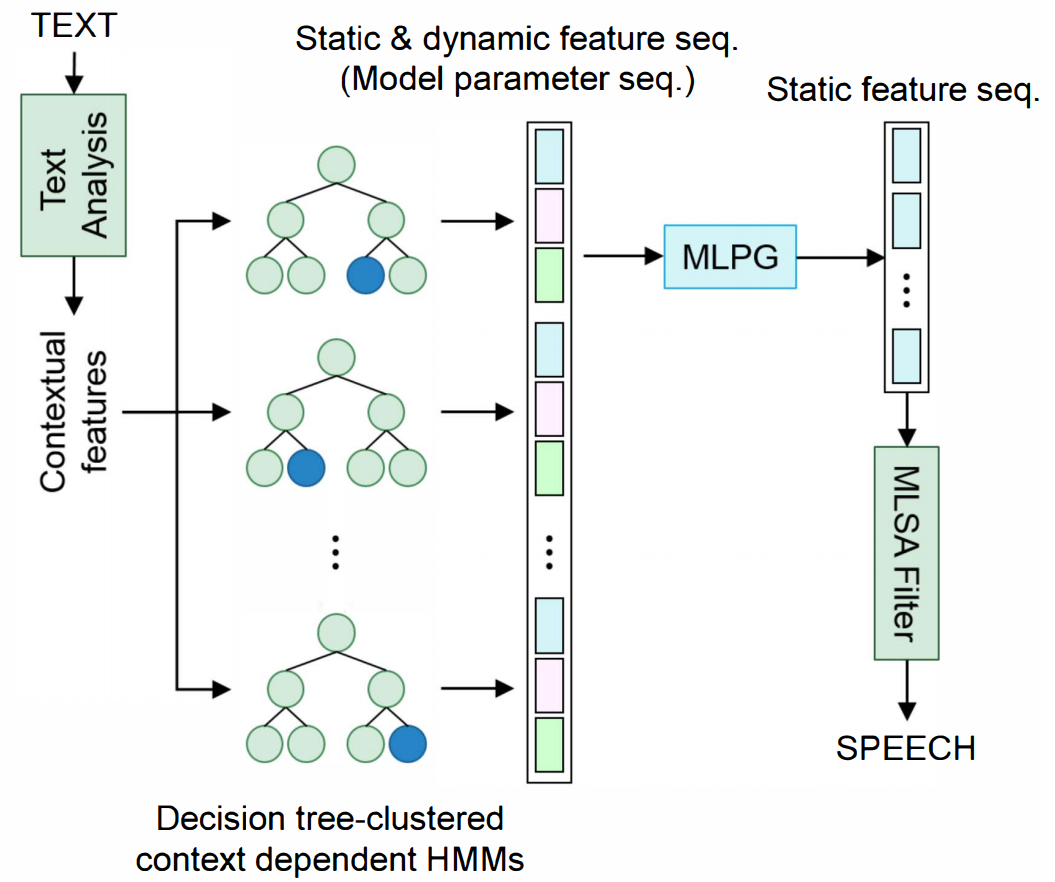
\includegraphics[width=\linewidth]{images/hmm_spss.png}
		\captionof{figure}{The general HMM-based TTS pipeline. Figure extracted from \citep{Hashimoto-2015}.}
		\label{hmm_spss_framework}
	\end{minipage}
	\hspace{.05\linewidth}
	\begin{minipage}{.45\linewidth}
		\centering
		\begin{tabular}{| l | c |}
			\hline
			Method & MOS \\
			\hline
			HMM+MLPG & 3.08 ($\pm$0.12) \\
			HMM+DNN & 2.86 ($\pm$0.12) \\
			\textbf{DNN+MLPG} & \textbf{3.53 ($\pm$0.12}) \\
			DNN+DNN & 3.17 ($\pm$0.12) \\
			\hline
		\end{tabular}
		\captionof{table}{MOS of the different methods explored in \citep{Hashimoto-2015}. The first line is the HMM-based framework. For the second and fourth line, the MLPG algorithm is replaced by a fully-connected neural network.}
		\label{hashimoto_results}
	\end{minipage}
\end{figure}

Improvements to this framework were later brought by feed-forward deep neural networks (DNN), as a result of progress in both hardware and software. \cite{SPSSDNN} proposes to replace entirely the decision tree-clustered HMMs in favor of a DNN. They argue for better data efficiency as the training set is no longer fragmented in different clusters of contexts. They demonstrate improvements over the speech quality with a number of parameters similar to that of the HMM-based approach. Later researches corroborate these findings \citep{OnTheTrainingAspects, Hashimoto-2015}. The MOS of different model combinations tried by \citep{Hashimoto-2015} are reported in Table \ref{hashimoto_results}

\citep{BDLSTMTTS} support that RNNs make natural acoustic models as they are able to learn a compact representation of complex and long-span functions. As RNNs are fit to generate temporally consistent series, the static features can directly be determined by the acoustic model, alleviating the need for dynamic features and MLPG. They compare networks of bidirectional LSTMs against the HMM and DNN based approaches described previously. Their A/B testing results are conclusive, we report them in figure \ref{dblstm_subjective}.

\begin{figure}[h]
	\centering
	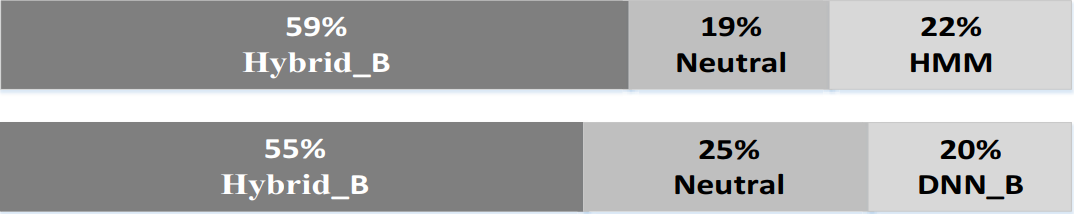
\includegraphics[width=0.6\linewidth]{images/bdlstm_subjective.png}
	\caption{A/B testing of the models. Hybrid\_B is a network with fully-connected and bidirectional LSTM layers. Figure extracted from \citep{BDLSTMTTS}.}
	\label{dblstm_subjective}
\end{figure}

The coming of WaveNet \citep{WaveNet} made a substantial breakthrough in TTS. WaveNet is a deep convolutional neural network that, for a raw audio waveform, models the distribution of a single sample given all previous ones. It is thus possible to directly generate audio by predicting samples one at a time in an autoregressive fashion. WaveNet leverages stacks of one-dimensional dilated convolutions with a dilation factor increasing exponentially with the layer depth, allowing for the very large receptive field and the strong nonlinearity needed to model raw audio. Conditioning the model on linguistic features is required to perform TTS. WaveNet acts thus both as an acoustic model and as a vocoder. Note that without the local conditioning, a trained WaveNet generates sound alike the training data but without structure or semantics (essentially babbling). 
The authors compare WaveNet to an older parametric approach and to a concatenative approach, the results are reported in Figure \ref{wavenet_results}. The parametric approach is an LSTM-based system while the other is an HMM-driven unit selection concatenative system (not detailed in this document). Notice how the results vary between US English and Mandarin Chinese, showing that TTS performance is not language agnostic.

\begin{figure}[h]
	\centering
	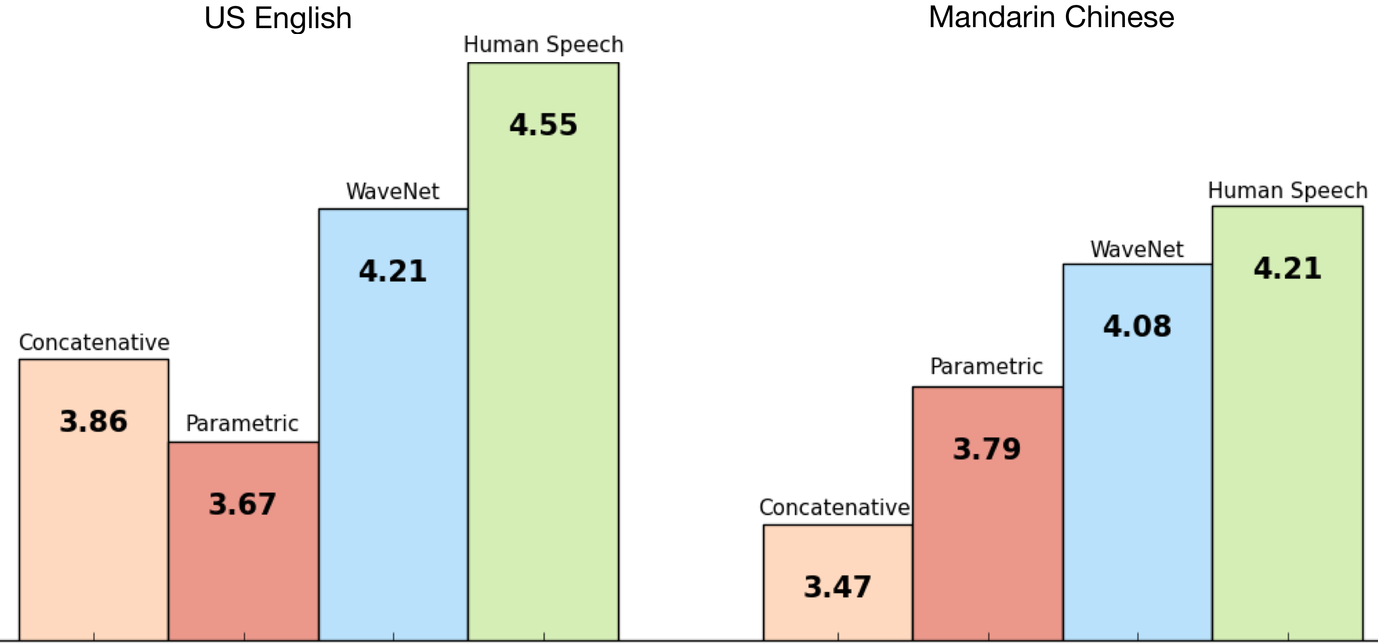
\includegraphics[width=.75\linewidth]{images/wavenet_results_chart.png}
	\caption[Figure]{MOS of WaveNet's performance compared with a parametric and concatenative approach, as well as with natural speech.\protect\footnotemark}
	\label{wavenet_results}
\end{figure}
\footnotetext{Figure extracted from \url{https://deepmind.com/blog/wavenet-generative-model-raw-audio/}}


%Deep Voice \citep{DeepVoice1} proposes a fully neural TTS framework that exploits WaveNet among other deep architectures. Deep Voice stands out by making use of only a few intermediate features: phonemes with stress annotations, phoneme durations,
%and F0. This has the advantage of making the framework easily transferable to new domains with little engineering effort as complex linguistic features need not be derived. The neural networks intervening in Deep Voice are: a grapheme-to-phoneme model that converts text to phonemes, a segmentation model that aligns a sequence of phonemes to an audio segment, a phoneme duration model that predicts the duration of each phoneme at generation time, a fundamental frequency model that predicts the V/UV flag with F0 values for voiced parts and finally, WaveNet which acts as an audio synthesis model. In all the works we presented previously, only the audio synthesis model was not manually engineered. While others have researched the use of neural networks for some of these components, Deep Voice is the first to simultaneously employ them all in a single framework. However, the grapheme-to-phoneme model is only used as a fallback for words not present in a phoneme dictionary. The roles and interactions of these components at training and inference time are shown in figure \ref{deep_voice_1_arch}. Deep Voice also improves on the inference time of WaveNet, with a speedup of up to 400. This allows for real-time or near real-time execution, with a tunable speed/quality trade-off. Deep Voice does not yield state of the art results but instead serves as groundwork for future researches. \color{red} discuss results \color{black}.
%
%\begin{figure}[h]
%	\centering
%	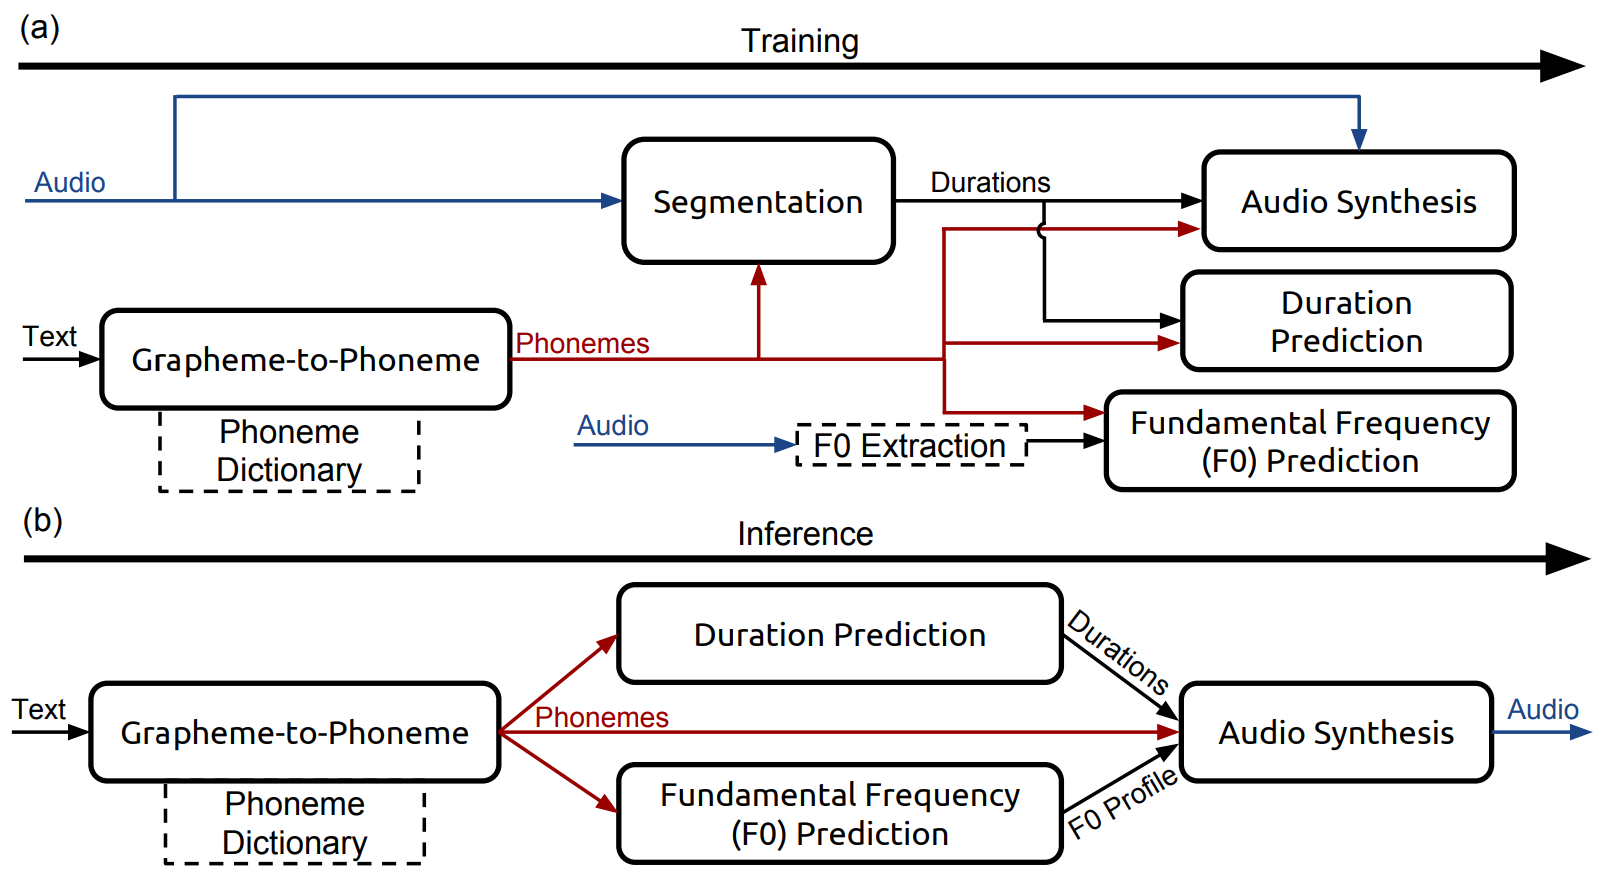
\includegraphics[width=.8\linewidth]{images/deep_voice_1_arch.png}
%	\caption{The training (a) and inference (b) procedure of Deep Voice. On the left of the image are the inputs, on the right are the outputs. Note that the segmentation model is only used for training.}
%	\label{deep_voice_1_arch}
%\end{figure}

% Up to 400x speedup on WaveNet
% Some previous research already use models to generate textual features
% No words with multiple pronunciations
% Natural MOS score when using ground truth F0 and durations
% Near real-time (accuracy/speed tradeoff)
% No diff when using original WaveNet

Follows Tacotron \citep{Tacotron1}, a sequence-to-sequence model that produces a spectrogram from a sequence of characters alone, further reducing the need for domain expertise. In this framework, the vocoder is the Griffin-Lim algorithm. Tacotron uses an encoder-decoder architecture where, at each step, the decoder operates on a weighted sum of the encoder outputs. This attention mechanism, described in \citep{Attention}, lets the network decide which steps of the input sequence are important with respect to each step of the output sequence. Tacotron achieves a MOS of 3.85 on a US English dataset, which is more than the 3.69 score obtained in the parametric approach of \citep{LSTM-RNN} but less than the 4.09 score obtained by the concatenative approach of \citep{ConcatenativeGoogle}. The authors mention that Tacotron is merely a step towards a better framework. Subsequently, Tacotron 2 is published \citep{Tacotron2}. The architecture of Tacotron 2 remains that of an encoder-decoder with attention although several changes to the type of layers are made. The main difference with Tacotron is the use of a modified WaveNet as vocoder. On the same dataset, Tacotron 2 achieves a MOS of 4.53, which compares to the 4.58 for human speech (the difference is not statistically significant), achieving the all-time highest MOS for TTS. With A/B testing, Tacotron 2 was found to be only slightly less preferred on average than ground truth samples. These ratings are shown in figure \ref{tacotron2_results}.

\begin{figure}[h]
	\centering
	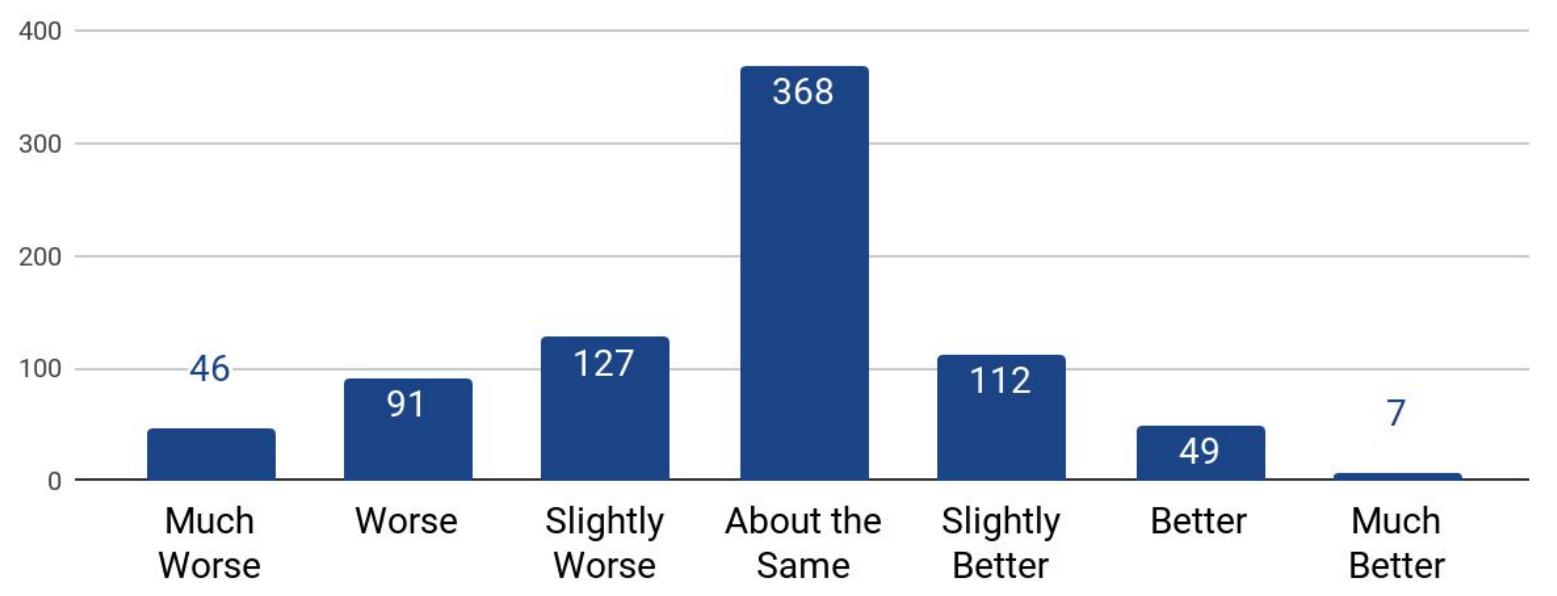
\includegraphics[width=.8\linewidth]{images/tacotron2_results.png}
	\caption{Preference ratings between Tacotron 2 and ground truth samples. There are 800 ratings from 100 items. The labels are expressed with respect to Tacotron 2. Figure extracted from \citep{Tacotron2}.}
	\label{tacotron2_results}
\end{figure}

\color{red} Efficient neural audio synthesis? \\ The plot summarizing everything \color{black}

\section{Related voice cloning methods}


% Wavenet:
%The output is a categorical distribution over sample values. For tractability reasons, the output signal is restricted to 256 discrete values that correspond to a $\mu$-law quantization, which is invertible. The MOS resulting from one of the experiments suggests that there is no statistically significant degradation in the naturalness of speech quantized in this manner. The architecture of WaveNet comes with several non-trivial components, described in later sections of this document \color{red}link to the section\color{black}. 
% The audio generated by WaveNet requires no post-processing other than the inversion of the $\mu$-law. 
%Furthermore, it allows for conditioning with respect to a vector constant at every timestep (global conditioning), which can be used to designate the speaker identity. The authors suggest that WaveNet is able to encode the embedding of several speakers seen in training with a shared internal representation. Speaker identities are given as a one-hot encoding. 

\section{Transfer Learning from Speaker Verification to Multispeaker Text-To-Speech Synthesis}
\subsection{Overview}
Our solution to real-time voice cloning is largely based on \citep{SV2TTS} (referred to as SV2TTS throughout this document). It describes an approach to zero-shot voice cloning that only requires 5 seconds of reference speech. This paper is only one of the many publications from the Tacotron series\footnote{\url{https://google.github.io/tacotron/}} authored at Google. Interestingly, the SV2TTS paper does not bring much innovation of its own, rather it is based on three major earlier works from Google: the GE2E loss \citep{GE2E}, Tacotron \citep{Tacotron1} and WaveNet \citep{WaveNet}. The complete framework is a three-stage pipeline, where the steps correspond to the models listed in order previously. Many of the current TTS tools and functionalities provided by Google, such as the Google assistant\footnote{\url{https://assistant.google.com/}} or the Google cloud services\footnote{\url{https://cloud.google.com/text-to-speech/}}, make use of these same models. While there are many open-source reimplementations of these models online, there is none of the SV2TTS framework to our knowledge (as of May 2019).

The three stages of the framework are as follows:
\begin{itemize}
	\item A speaker encoder that derives an embedding from the short utterance of a single speaker. The embedding is a meaningful representation of the voice of the speaker, such that similar voices are close in latent space. This model is described in \citep{GE2E} (referred as GE2E throughout this document) and \citep{TE2E}.
	\item A synthesizer that, conditioned on the embedding of a speaker, generates a spectrogram from a text. This model is the popular Tacotron 2 \citep{Tacotron2} without WaveNet (which is often referred to as just Tacotron due to its similarity to the first iteration).
	\item A vocoder that infers an audio waveform from the spectrograms generated by the synthesizer. The authors used WaveNet \citep{WaveNet} as a vocoder, effectively reapplying the entire Tacotron 2 framework.
\end{itemize}
At inference time, the speaker encoder is fed a short reference utterance of the speaker to clone. It generates an embedding that is used to condition the synthesizer, and a text processed as a phoneme sequence is given as input to the synthesizer. The vocoder takes the output of the synthesizer to generate the speech waveform. This is illustrated in figure \ref{sv2tts_framework}.

\begin{figure}[h]
	\centering
	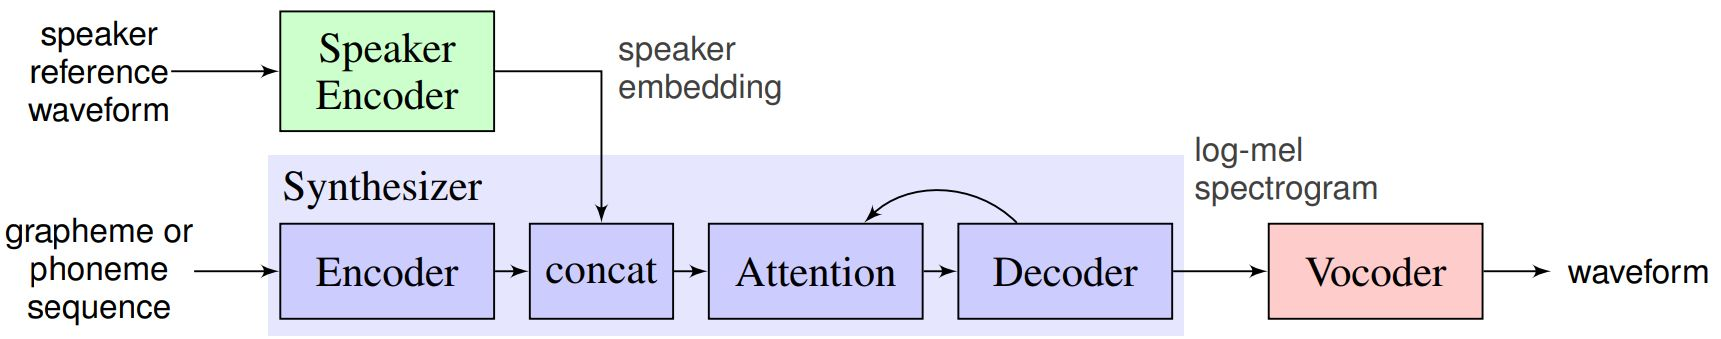
\includegraphics[width=\linewidth]{images/sv2tts_framework.jpg}
	\caption{The SV2TTS framework during inference. The blue blocks represent a high-level view of the Tacotron architecture modified to allow conditioning on a voice. Figure extracted from \citep{SV2TTS}.}
	\label{sv2tts_framework}
\end{figure}

A particularity of the SV2TTS framework is that all models can be trained separately and on distinct datasets. For the encoder, one seeks to have a model that is robust to noise and able to capture the many characteristics of the human voice. Therefore, a large corpus of many different speakers would be preferable to train the encoder, without any strong requirement on the noise level of the audios. Additionally, the encoder is trained with the GE2E loss which requires no labels other than the speaker identity. With GE2E, the task to be learned by the model is a speaker verification task, which by itself has little to do with voice cloning. However, the task is stipulated in way that the network will output an embedding that is a meaningful representation of the voice of the speaker. This embedding is suitable for conditioning the synthesizer on a voice, hence the name of the paper: "Transfer Learning from Speaker Verification to Multispeaker Text-To-Speech Synthesis". For the datasets of the synthesizer and the vocoder, transcripts are required and the quality of the generated audio can only be as good as that of the data. Higher quality and annotated datasets are thus required, which often means they are smaller in size.

%In subsection \ref{problem_definition}, we formally define the task that SV2TTS aims to solve. In the remaining subsections, we present the three parts of the framework as described in \citep{SV2TTS}.


\subsection{Problem definition} \label{problem_definition}
\newcommand{\vx}{\mathbf{x}}
\newcommand{\vu}{\mathbf{u}}
\newcommand{\ve}{\mathbf{e}}
\newcommand{\vt}{\mathbf{t}}
\newcommand{\vc}{\mathbf{c}}
\newcommand{\vw}{\mathbf{w}}
\newcommand{\ms}{\mathbf{S}}
\newcommand{\enc}{\mathcal{E}}
\newcommand{\syn}{\mathcal{S}}
\newcommand{\voc}{\mathcal{V}}
Consider a dataset of utterances grouped by their speaker. We denote the $j$th utterance of the $i$th speaker as $\vu_{ij}$. Utterances are in the waveform domain. We denote by $\vx_{ij}$ the log-mel spectrogram of the utterance $\vu_{ij}$. A log-mel spectrogram is a deterministic, non-invertible (lossy) but derivable function that extracts speech features from a waveform, so as to handle audio in a more tractable fashion in machine learning.

The encoder $\enc$ computes the embedding $\ve_{ij} = \enc(\vx_{ij}; \vw_\enc)$ corresponding to the utterance $\vu_{ij}$, where $\vw_\enc$ are the parameters of the encoder. Additionally, the authors define a speaker embedding as the centroid of the embedding of the speaker's utterances:
\begin{equation}\label{speaker_embedding}
\vc_i=\frac{1}{n}\sum_{j}^{n}\ve_{ij}
\end{equation}

The synthesizer $\syn$, parametrized by $\vw_\syn$, is tasked to approximate $\vx_{ij}$ given $\vc_i$ and $\vt_{ij}$, the transcript of utterance $\vu_{ij}$. We have $\hat\vx_{ij} = \syn(\vc_i, \vt_{ij}; \vw_\syn)$. In our implementation, we directly use the utterance embedding rather than the speaker embedding (we motivate this choice in section \ref{synthesizer}), giving instead $\hat\vx_{ij} = \syn(\vu_{ij}, \vt_{ij}; \vw_\syn)$.

Finally, the vocoder $\voc$, parametrized by $\vw_\voc$, is tasked to approximate $\vu_{ij}$ given $\hat\vx_{ij}$. We have $\hat\vu_{ij} = \voc(\hat\vx_{ij}; \vw_\voc)$.

One could train this framework in an end-to-end fashion with the following objective function:
$$ min_{\vw_\enc, \vw_\syn, \vw_\voc} L_\voc(\vu_{ij}, \voc(\syn(\enc(\vx_{ij}; \vw_\enc), \vt_{ij}; \vw_\syn); \vw_\voc)) $$
Where $L_\voc$ is a loss function in the waveform domain. This approach has drawbacks:
\begin{itemize}
	\item It requires training all three models on a same dataset, meaning that this dataset would ideally need to meet the requirements for all models: a large number of speakers for the encoder but at the same time transcripts for the synthesizer and a low level noise for the synthesizer and somehow an average noise level for the encoder (so as to be able to handle noisy input speech). These conflicts are problematic and would lead to training models that could perform better if trained separately on distinct datasets. Specifically, a small dataset will likely lead to poor generalization and thus poor zero-shot performance.
	\item The convergence of the combined model could be very hard to reach. In particular, the Tacotron synthesizer typically takes a significant time before producing correct alignments (see \rw).
\end{itemize}

An evident way of addressing the second issue is to separate the training of the synthesizer and of the vocoder. Assuming a pretrained encoder, the synthesizer can be trained to directly predict the mel spectrograms of the target audio:
$$ min_{\vw_\syn} L_\syn(\vx_{ij}, \syn(\ve_{ij}, \vt_{ij}; \vw_\syn)) $$
Where $L_\syn$ is a loss function in the time-frequency domain. 

The vocoder is then trained directly on the spectrograms. Note that both the approaches of training on ground truth spectrograms or on synthesizer-generated spectrograms are valid (see \rw). The latter requires a pretrained synthesizer.
$$ min_{\vw_\voc} L_\voc(\vu_{ij}, \voc(\vx_{ij}; \vw_\voc)) \ \ \text{or} \ \ 
   min_{\vw_\voc} L_\voc(\vu_{ij}, \voc(\hat\vx_{ij}; \vw_\voc)) $$

Remains the optimization of the speaker encoder. Unlike the synthesizer and the vocoder, the encoder does not have labels to be trained on. The task is lousily defined as producing "meaningful" embeddings that characterize the voice in the utterance. One could conceive of a way to train the speaker encoder as an autoencoder, but it would require the corresponding upsampling model to be made aware of the text to predict. Either the dataset is constrained to a same sentence, either one needs transcripts and the upsampling model is the synthesizer. In both cases the quality of the training is impaired by the dataset and unlikely to generalize well. Fortunately, the GE2E loss \citep{GE2E} brings a solution to this problem and allows to train the speaker encoder independently of the synthesizer. This is described in section \ref{speaker_encoder}. 

\begin{figure}[h]
	\centering
	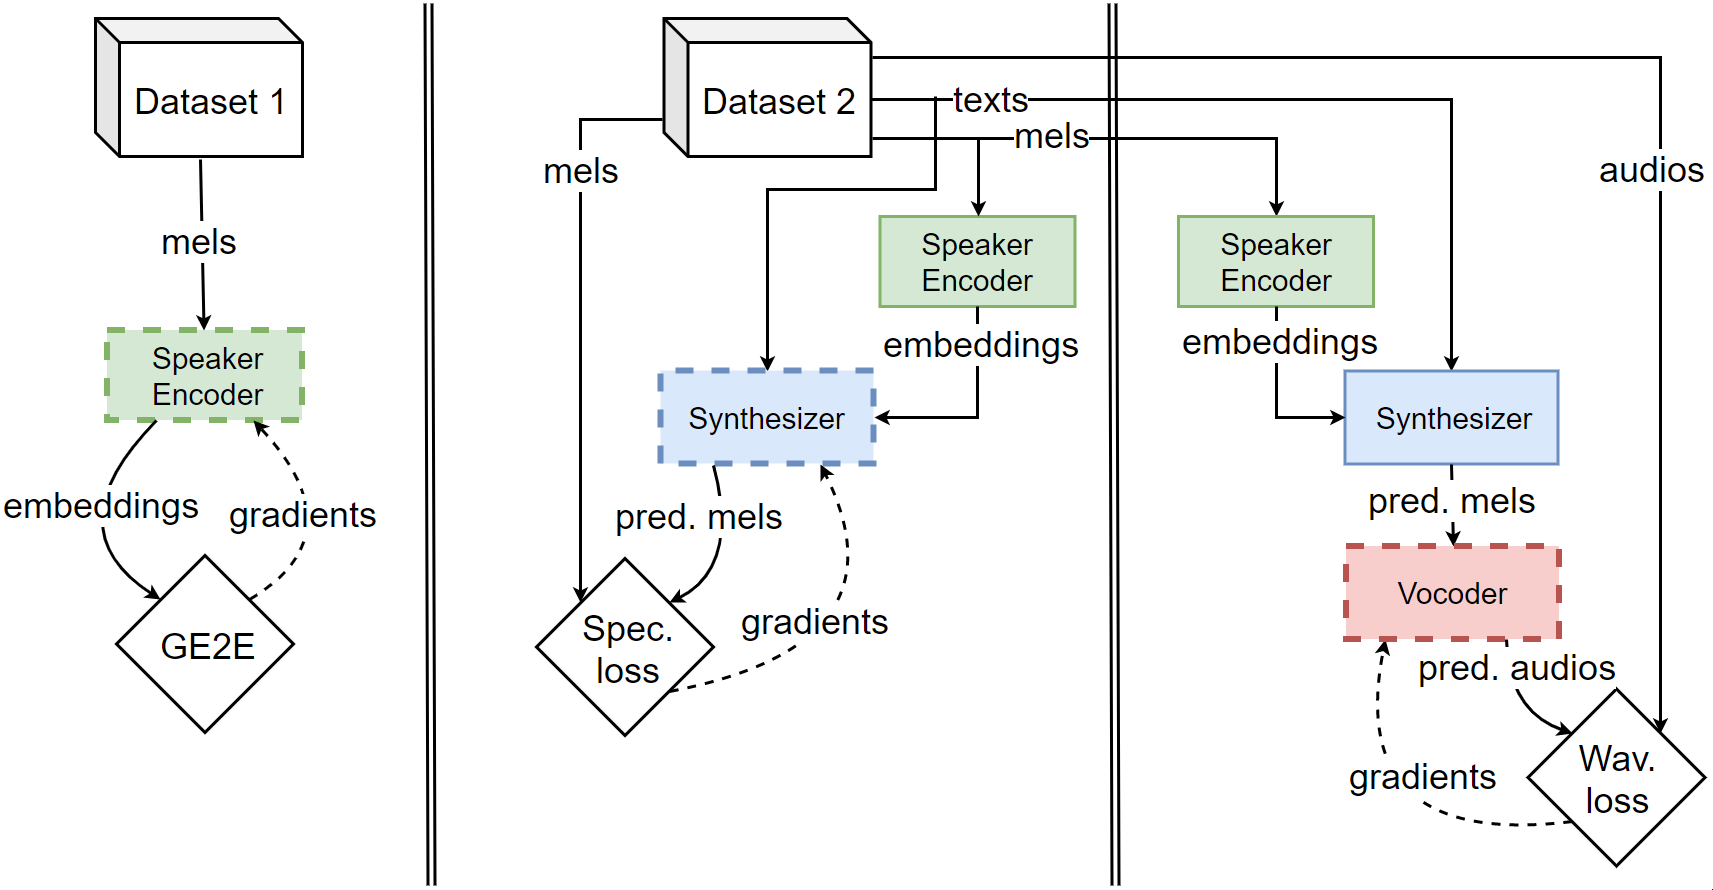
\includegraphics[width=\linewidth]{images/sv2tts_training.png}
	\caption{The sequential three-stage training of SV2TTS (following our choices of implementation). Models with solid contour lines are frozen. Note that the mel spectrograms fed to the speaker encoder and those used as target for the synthesizer are created with different parameters.}
	\label{sv2tts_training}
\end{figure}

While all parts of the framework are trained separately, there is still the requirement for the synthesizer to have embeddings from a trained encoder and for the vocoder to have mel spectrograms from a trained synthesizer (if not training on ground truth spectrogram). Figure \ref{sv2tts_training} illustrates how each model depends on the previous one for training. The speaker encoder needs to generalize well enough to produce meaningful embeddings on the dataset of the synthesizer; and even when trained on a common dataset, it still has to be able to operate in a zero-shot setting at inference time. 

\subsection{Speaker encoder} \label{speaker_encoder}
The encoder model and its training procedure are described over several papers \citep{SV2TTS, GE2E, TE2E}. We reproduced this model with a PyTorch implementation of our own. We synthesize the parts that are pertinent to SV2TTS as well as our choices of implementation.

\subsubsection{Model architecture}
The model is a 3-layer LSTM with 768 hidden nodes followed by a projection layer of 256 units. While there is no reference in any of the papers as to what a projection layer is, the intuition is that it is simply a 256 outputs fully-connected layer per LSTM that is repeatedly applied to every output of the LSTM. When we first implemented the speaker encoder, we directly used 256 units LSTM layers instead, for the sake of quick prototyping, simplicity and for a lighter training load. This last part is important, as the authors have trained their own model for 50 million steps (although on a larger dataset), which is technically difficult for us to reproduce. We found this smaller model to perform extremely well, and we haven't found the time to train the larger version later on. \color{red} move to experiments? \color{black}

The inputs to the model are 40-channels log-mel spectrograms with a 25ms window width and a 10ms step. The output is the L2-normalized hidden state of the last layer, which is a vector of 256 elements. Our implementation also features a ReLU layer before the normalization, with the goal in mind to make embeddings sparse and thus more easily interpretable.

\subsubsection{Generalized End-to-End loss}
The speaker encoder is trained on a speaker verification task. Speaker verification is a typical application of biometrics where the identity of a person is verified through their voice. A template is created for a person by deriving their speaker embedding (see equation \ref{speaker_embedding}) from a few utterances. This process is called enrollment. At runtime, a user identifies himself with a short utterance and the system compares the embedding of that utterance with the enrolled speaker embeddings. Above a given similarity threshold, the user is identified. The GE2E loss simulates this process to optimize the model. 

At training time, the model computes the embeddings $\ve_{ij}\ (1 \leq i \leq N, 1 \leq j \leq M)$ of $M$ utterances of fixed duration from $N$ speakers. A speaker embedding $\vc_i$ is derived for each speaker: $\vc_i=\frac{1}{M}\sum_{j}^{M}\ve_{ij}\ (1 \leq i \leq N)$. The similarity matrix $\ms_{ij,k}$ is the result of the two-by-two comparison of all embeddings $\ve_{ij}$ against every speaker embedding $\vc_{k}\ (1 \leq k \leq N)$ in the batch. This measure is the scaled cosine similarity:

\begin{equation} \label{similarity_simple}
	\ms_{ij,k} = w \cdot cos(\ve_{ij}, \vc_{k}) + b = w \cdot \ve_{ij} \cdot ||\vc_{k}||_2 + b
\end{equation}

where $w$ and $b$ are learnable parameters. This entire process is illustrated in figure \ref{sim_matrix}.  From a computing perspective, the cosine similarity of two L2-normed vectors is simply their dot product, hence the rightmost hand side of equation \ref{similarity_simple}. An optimal model is expected to output high similarity values when an utterance matches the speaker $(i = k)$ and lower values elsewhere $(i \neq k)$. To optimize in this direction, the loss is the sum of row-wise softmax losses.

\begin{figure}[h]
	\centering
	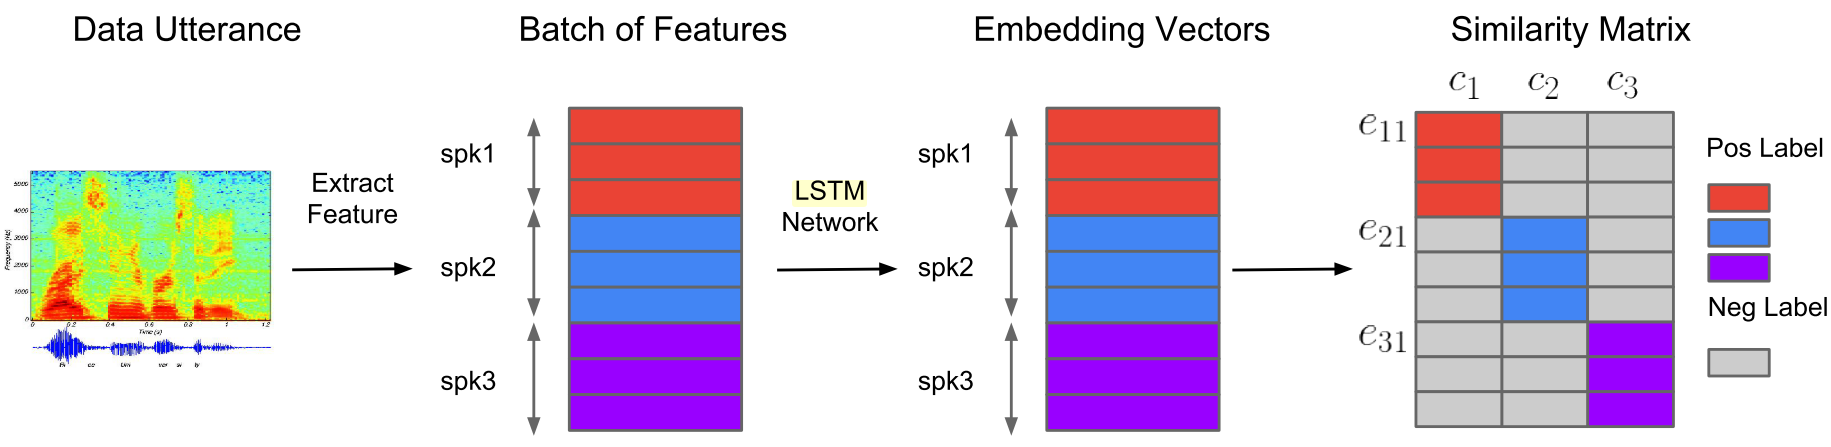
\includegraphics[width=\linewidth]{images/sim_matrix.png}
	\caption{The construction of the similarity matrix at training time. This figure is extracted from \citep{GE2E}.}
	\label{sim_matrix}
\end{figure}

Note that each utterance $\ve_{ij}$ is included in the centroid $\vc_{i}$ of the same speaker when computing the loss. This creates a bias towards the correct speaker independently of the accuracy of the model. To prevent this, an utterance that is compared against its own speaker's embedding will be removed from the computation of the speaker embedding. The similarity matrix is then defined as:
\begin{equation} \label{similarity_exclusive}
\ms_{ji,k} =
\begin{cases}
w\cdot \cos(\ve_{ij}, \vc_i^{(-j)})+b & \text{if} \quad i=k \\
w\cdot \cos(\ve_{ij}, \vc_k)+b & \text{otherwise}.
\end{cases}
\end{equation}
where the exclusive centroids $\vc_{i}^{(-j)}$ are defined as:
\begin{equation} \label{exclusive_centroid}
\vc_{i}^{(-j)} = \frac{1}{M-1}\sum_{\substack{m=1\\m\neq j}}^{M}\ve_{im}
\end{equation}

The fixed duration of the utterances in a training batch is of 1.6 seconds. These utterances are partial utterances sampled from the longer complete utterances in the dataset. While the model architecture is able to handle inputs of variable length, it is reasonable to expect that it performs best with utterances of the same duration as those seen in training. Therefore, at inference time an utterance is split in segments of 1.6 seconds overlapping by 50\%, and the encoder forwards each segment individually. The resulting outputs are averaged then normalized to produce the utterance embedding. This is illustrated in figure \ref{encoder_inference}. Curiously, the authors of SV2TTS advocate for 800ms windows at inference time but still 1.6 seconds ones during training. We prefer to keep 1.6 seconds for both, as is done in GE2E.

\begin{figure}[h]
	\centering
	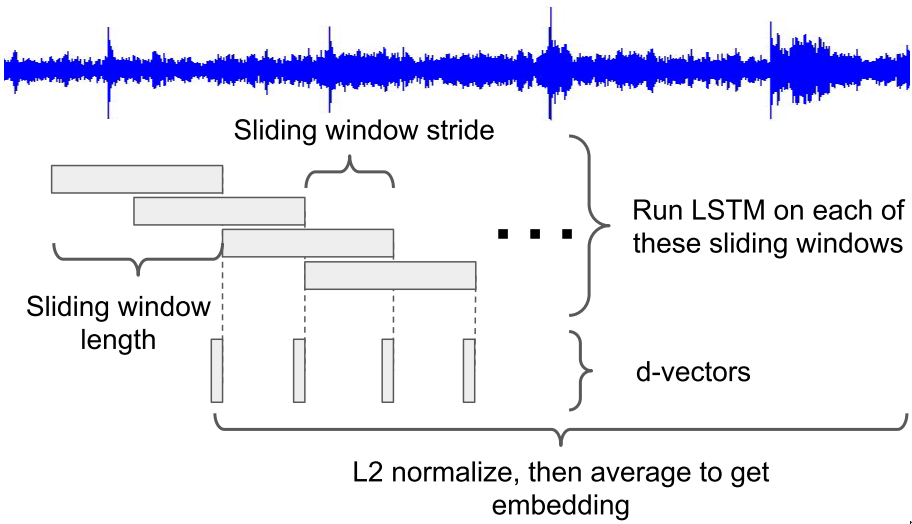
\includegraphics[width=0.65\linewidth]{images/encoder_inference.png}
	\caption{Computing the embedding of a complete utterance. The d-vectors are simply the unnormalized outputs of the model. This figure is extracted from \citep{GE2E}.}
	\label{encoder_inference}
\end{figure}

The authors use $N = 64$ and $M = 10$ as parameters for the batch size. When enrolling a speaker in a practical application, one should expect to have several utterances from each user but likely not an order of magnitude above that of 10, so this choice is reasonable. As for the number of speakers, it is good to observe that the time complexity of computing the similarity matrix is $O(N^2M)$. Therefore this parameter should be chosen not too large so as to not slow down substantially the training, as opposed to simply picking the largest batch size that fits on the GPU. It is still of course possible to parallelize multiple batches on the same GPU while synchronizing the operations across batches for efficiency. We found it particularly important to vectorize all operations when computing the similarity matrix, so as to minimize the number of GPU transactions.

\subsubsection{Experiments}
To avoid segments that are mostly silent when sampling partial utterances from complete utterances, we use the webrtcvad\footnote{\url{https://github.com/wiseman/py-webrtcvad}} python package to perform Voice Activity Detection (VAD). This yields a binary flag over the audio corresponding to whether or not the segment is voiced. We perform a moving average on this binary flag to smooth out short spikes in the detection, which we then binarize again. Finally, we perform a dilation on the flag with a kernel size of $s + 1$, where $s$ is the maximum silence duration tolerated. The audio is then trimmed of the unvoiced parts. We found the value $s=0.2$s to be a good choice that retains a natural speech prosody. This process is illustrated in figure \ref{encoder_preprocess_vad}. A last preprocessing step applied to the audio waveforms is normalization, to make up for the varying volume of the speakers in the dataset.

\begin{figure}[h]
	\centering
	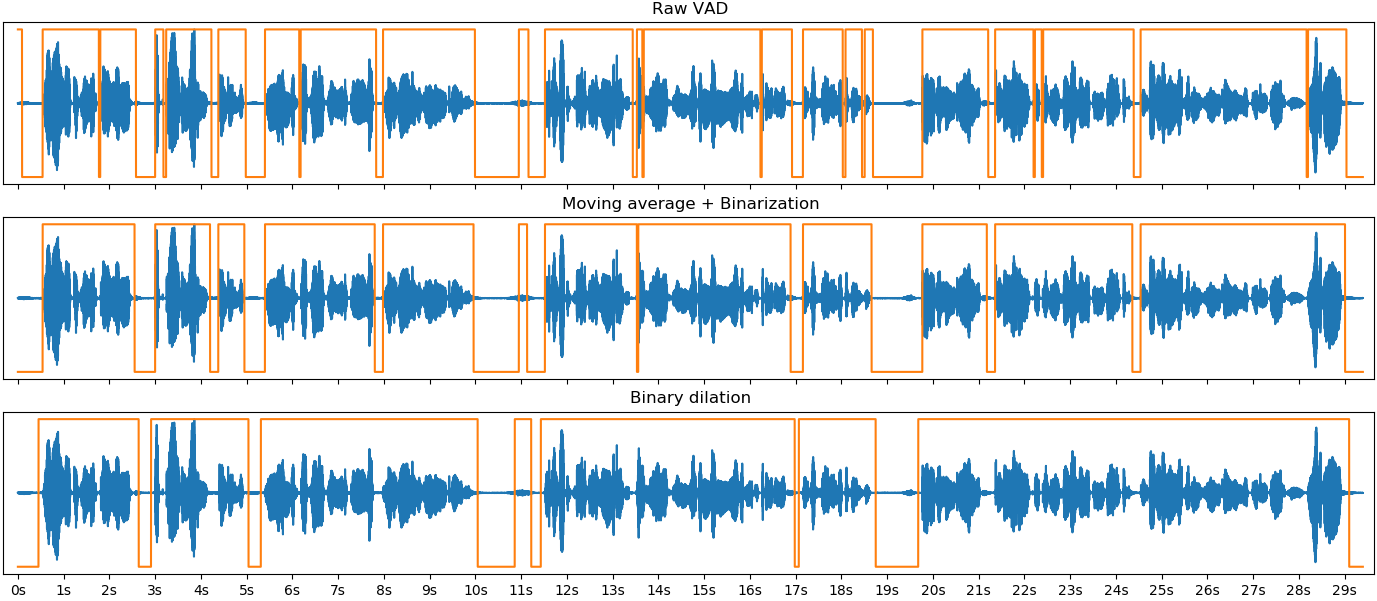
\includegraphics[width=\linewidth]{images/encoder_preprocess_vad.png}
	\caption{The steps to silence removal with VAD, from top to bottom. The orange line is the binary voice flag where the upper value means that the segment is voiced, and unvoiced when lower.}
	\label{encoder_preprocess_vad}
\end{figure}

The authors combined several noisy datasets to make for a large corpus of speech of quality similar to what is found in the wild. These datasets are LibriSpeech \citep{LibriSpeech}, VoxCeleb1 \citep{VoxCeleb1}, VoxCeleb2 \citep{VoxCeleb2} and an internal dataset, to which we do not have access. LibriSpeech is a corpus of audiobooks making up for 1000 hours of audio from 2400 speakers, split equally in two sets "clean" and "other". The clean set is supposedly made up of cleaner speech than the other set, even though some parts of the clean set still contain a lot of noise \citep{LibriTTS}. VoxCeleb1 and VoxCeleb2 are made up from audio segments extracted from youtube videos of celebrities (often in the context of an interview). VoxCeleb1 has 1.2k speakers, while VoxCeleb2 has about 6k. Both these datasets have non-English speakers. We used heuristics based on the nationality of the speaker to filter non-English ones out of the training set in VoxCeleb1, but couldn't apply those same heuristics to VoxCeleb2 as the nationality is not referenced in that set. Note that it is unclear without experimentation as to whether having non-English speakers hurts the training of the encoder (the authors make no note of it either). All these datasets are sampled at 16kHz.

The authors test different combinations of these datasets and observe the effect on the quality of the embeddings. They adjust the output size of LSTM model (the size of the embeddings) to 64 or 256 according to the number of speakers. They evaluate the subjective naturalness and similarity with ground truth of the speech generated by a synthesizer trained from the embeddings produced by each model. They also report the equal error rate of the encoder on speaker verification, which we discuss later in this section. These results can be found in Table \ref{encoder_training_datasets}.

\begin{table}[h]
	\begin{center}
		\begin{footnotesize}
			\begin{tabular}{cccccc}
				\toprule
				Training Set & Speakers & Embedding Dim & Naturalness & Similarity & SV-EER \\ \midrule
				LS-Clean &            1.2K & 64 & $3.73 \pm 0.06$ &
				$2.23 \pm 0.08$
				& 16.60\%\\
				LS-Other &            1.2K & 64 & $3.60 \pm 0.06$ &
				$2.27 \pm 0.09$
				& 15.32\% \\
				LS-Other+VC &            2.4K & 256 & $3.83 \pm 0.06$ &
				$2.43 \pm 0.09$
				& 11.95\% \\
				$\bullet$ LS-Other+VC+VC2 &            8.4K & 256 & $3.82 \pm 0.06$ &
				$2.54 \pm 0.09$ 
				& 10.14\% \\
				Internal  & 18K & 256 & $4.12 \pm 0.05$ &
				$3.03 \pm 0.09$
				& 5.08\% \\
				\bottomrule
			\end{tabular}
		\end{footnotesize} 
	\end{center}
	\caption{Training of the speaker encoder on different datasets, from \citep{SV2TTS}. LS is LibriSpeech and VC is VoxCeleb. The synthesizers are trained on LS-Clean and evaluated on a test set. The line with a bullet is the implementation we aim to reproduce.}
	\label{encoder_training_datasets}
\end{table}

These results indicate that the number of speakers is strongly correlated with the good performance of not only the encoder on the verification task, but also of the entire framework on the quality of the speech generated and on its ability to clone a voice. The small jump in naturalness, similarity and EER gained by including VoxCeleb2 could indicate that the variation of languages is hurting the training. The internal dataset of the authors is a proprietary voice search corpus from 18k English speakers. The encoder trained on this dataset performs significantly better, however we only have access to public datasets. We thus proceed with LibriSpeech-Other, VoxCeleb1 and VoxCeleb2.

We train the speaker encoder for one million steps. To monitor the training we report the EER and we observe the ability of the model to cluster speakers. We periodically sample a batch of 10 speakers with 10 utterances each, compute the utterance embeddings and projecting them in a two-dimensional space with UMAP \citep{UMAP}. As embeddings of different speakers are expected to be further apart in the latent space than embeddings from the same speakers, it is expected that clusters of utterances from a same speaker form as the training progresses. We report our UMAP projections in figure \ref{training_umap}, where this behaviour can be observed.

\begin{figure}[h]
	\centering
	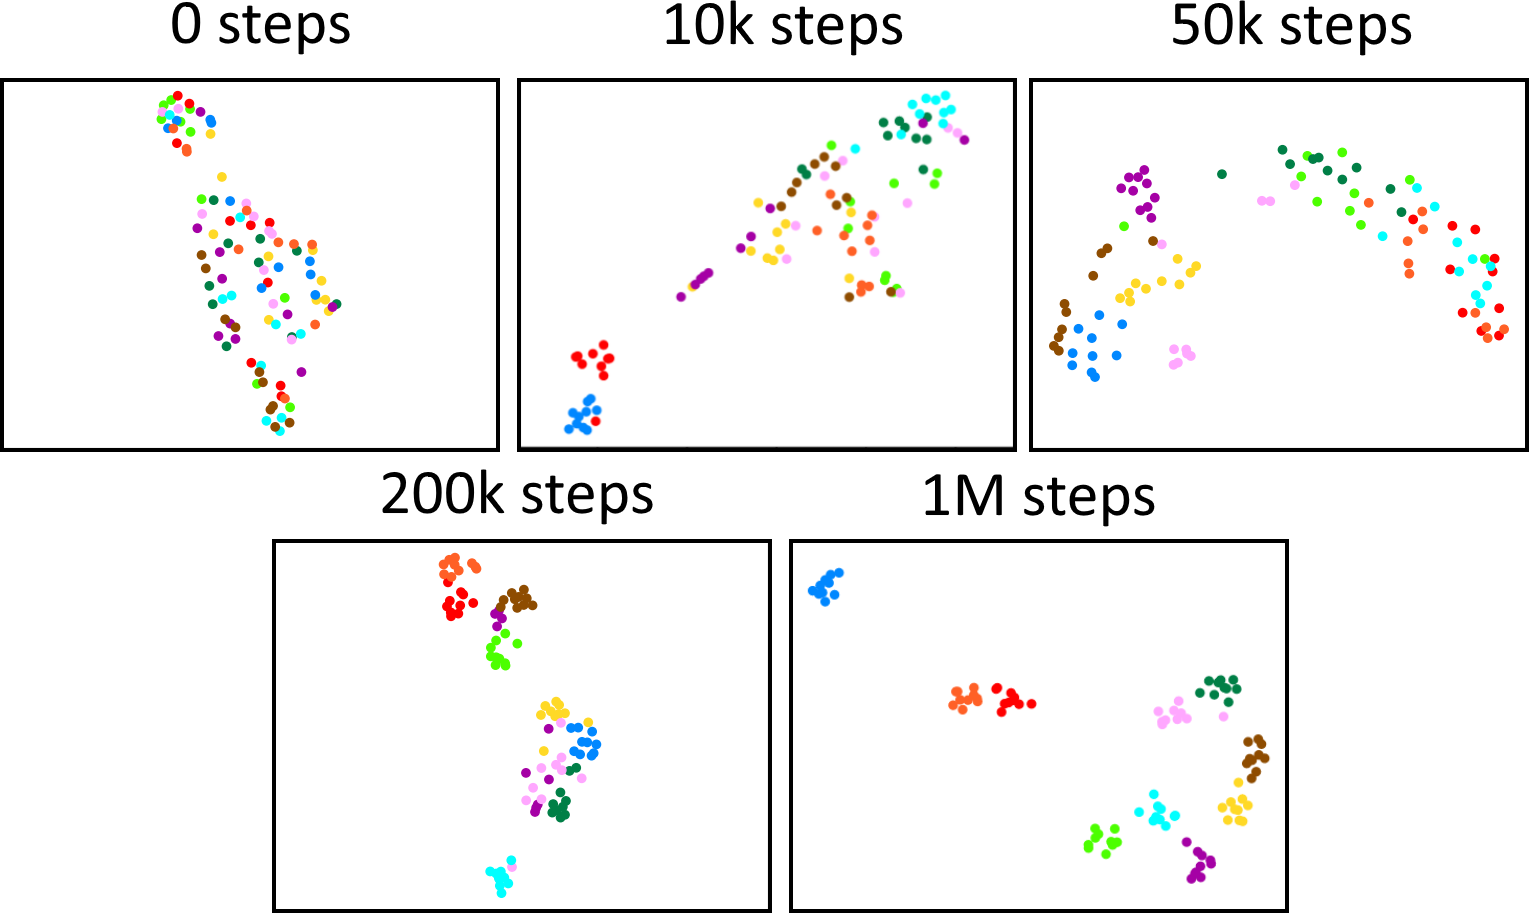
\includegraphics[width=\linewidth]{images/training_umap.png}
	\caption{UMAP projections of utterance embeddings from randomly selected batches from the train set at different iterations of our model. Utterances from the same speaker are represented by a dot of the same color. We specifically omit to pass labels to UMAP, so the clustering is entirely done by the model.}
	\label{training_umap}
\end{figure}

As mentioned before, the authors have trained their model for 50 million steps on their proprietary dataset. While both our dataset and our model are smaller, our model still hasn't converged at 1 million steps. The loss decreases steadily with little variance and can still decrease more, but we are bound by the time.

\color{red} loss plot + test set? + EER \color{black}



\subsection{Synthesizer} \label{synthesizer}
The synthesizer is Tacotron 2 without Wavenet \citep{WaveNet}. We use an open-source implementation\footnote{\url{https://github.com/Rayhane-mamah/Tacotron-2}} of Tacotron 2 from which we strip Wavenet and implement the modifications added by SV2TTS.

\subsubsection{Model architecture}
We briefly present the top-level architecture of the modified Tacotron 2 without Wavenet (which we'll refer to as simply Tacotron). For further details, we invite the reader to take a look at the Tacotron papers \citep{Tacotron2, Tacotron1}.

Tacotron is a recurrent sequence-to-sequence model that predicts a mel spectrogram from text. It features an encoder-decoder structure (not to be mistaken with the speaker encoder of SV2TTS) that is bridged by a location-sensitive attention mechanism \citep{Attention2}. Individual characters from the text sequence are first embedded as vectors. Convolutional layers follow, so as to increase the information span of a single encoder frame. These frames are passed through a bidirectional LSTM to produce the encoder output frames. This is where SV2TTS brings a modification to the architecture: a speaker embedding is concatenated to every frame output by the encoder. The attention mechanism attends to the encoder output frames to generate the decoder input frames. Each decoder input frame is concatenated with the previous decoder frame output passed through a pre-net, making the model autoregressive. This concatenated vector goes through two unidirectional LSTM layers before being projected to a single mel spectrogram frame. Another projection of the same vector to a scalar allows the network to predict on its own that it should stop generating frames by emitting a value above a certain threshold. The entire sequence of frames is passed through a residual post-net before it becomes the mel spectrogram. This architecture is represented in figure \ref{tacotron2_arch}.

\begin{figure}[h]
	\centering
	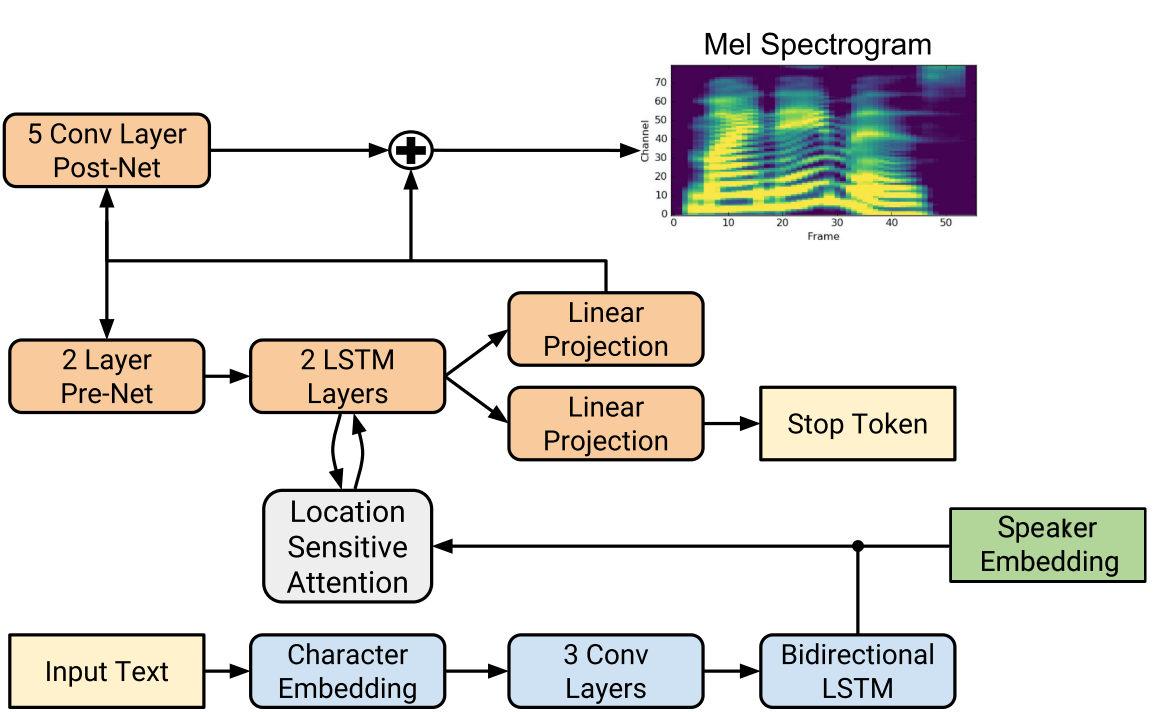
\includegraphics[width=0.7\linewidth]{images/tacotron2_arch.png}
	\caption{The modified Tacotron architecture. The blue blocks correspond to the encoder and the orange ones to the decoder. This figure was extracted from \citep{Tacotron2} and modified.}
	\label{tacotron2_arch}
\end{figure}


A noteworthy property of presenting the embedding at every encoder step is that it allows to change a voice through a sentence, e.g. by morphing a voice to another with a linear interpolation between their respective embeddings.

The target mel spectrograms for the synthesizer present more features than those used for the speaker encoder. They are computed from a 50ms window with a 12.5ms step and have 80 channels. The input texts are not processed for pronunciation in our implementation.

\subsubsection{Experiments}
In SV2TTS, the authors consider two datasets for training both the synthesizer and the vocoder. These are LibriSpeech-Clean which we have mentioned earlier and VCTK\footnote{\url{https://homepages.inf.ed.ac.uk/jyamagis/page3/page58/page58.html}} which is a corpus of only 109 native English speakers recorded with professional equipment. The speech in VCTK is sampled at 48kHz and downsampled to 24kHz in their experiments, which is still higher than the 16kHz sampling of LibriSpeech. They find that a synthesizer trained on LibriSpeech generalizes better than on VCTK when it comes to similarity but not naturalness. They assess this by training the synthesizer on one set, and testing it on the other. These results are in Table \ref{libri_vctk_cross}. We decided to work with the dataset that would offer the best voice cloning similarity on unseen speakers, and therefore picked LibriSpeech. We have also tried using the newer LibriTTS~\citep{LibriTTS} dataset created by the Tacotron team. This dataset is a cleaner version of the whole LibriSpeech corpus with noisy speakers pruned out, a higher sampling rate of 24kHz and the punctuation that LibriSpeech lacks. Unfortunately, the synthesizer could not produce meaningful alignments on this dataset for reasons we ignore. We kept the original LibriSpeech dataset instead.

\begin{table}[h]
	\begin{center}
		\begin{small}
			\begin{tabular}{cccc}
				\toprule
				Synthesizer Training Set & Testing Set & Naturalness & Similarity \\
				\midrule
				VCTK & LibriSpeech & $4.28 \pm 0.05$ & $1.82 \pm 0.08$ \\
				LibriSpeech & VCTK & $4.01 \pm 0.06$ & $2.77 \pm 0.08$ \\
				\bottomrule
			\end{tabular}
		\end{small}
	\end{center}
	\caption{Cross-dataset evaluation on naturalness and speaker similarity for unseen speakers. This table is extracted from \citep{SV2TTS}}
	\label{libri_vctk_cross}
\end{table}

Following the preprocessing recommendations of the authors, we use an Automatic Speech Recognition (ASR) model to force-align the LibriSpeech transcripts to text. We found the Montreal Forced Aligner\footnote{\url{https://montreal-forced-aligner.readthedocs.io/en/latest/}} to perform well on this task. We've also made a cleaner version of these alignments public\footnote{\url{https://github.com/CorentinJ/librispeech-alignments}} to save some time for other users in need of them. With the audio aligned to the text, we split utterances on silences longer than 0.4 seconds. This helps the synthesizer to converge, both because of the removal of silences in the target spectrogram, but also due to the reduction of the median duration of the utterances in the dataset, as shorter sequences offer less room for timing errors. We ensure that utterances are not shorter than 1.6 seconds, the duration of partial utterances used for training the encoder, and not longer than 11.25 seconds so as to save GPU memory for training. We do not split on a silence that would create an utterance too short or too long if possible. The distribution of the length of the utterances in the dataset is plotted in figure \ref{librispeech_durations}. Note how long silences already account for 64 hours (13.7\%) of the dataset.

\begin{figure}[h]
	\centering
	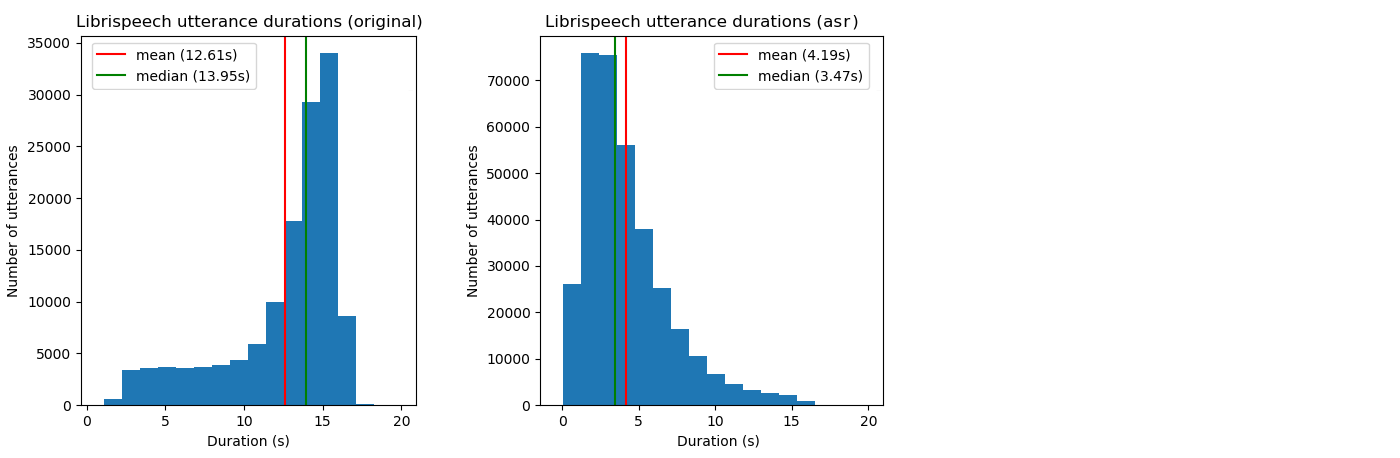
\includegraphics[width=\linewidth]{images/librispeech_durations.png}
	\caption{(left) Histogram of the duration of the utterances in LibriSpeech-Clean, (middle) after splitting on silences, (right) after constraining the length and readjusting the splits.}
	\label{librispeech_durations}
\end{figure}

Isolating the silences with force-aligning the text to the utterances additionally allows to create a profile of the noise for all utterances of the same speaker. We found a Fourier-analysis based noise removal algorithm to perform well on this task, but unfortunately could not reimplement this algorithm in our preprocessing pipeline.

In SV2TTS, the embeddings used to condition the synthesizer at training time are speaker embeddings. We argue that utterance embeddings of the same target utterance make for a more natural choice. At inference time, utterance embeddings are used. While the space of utterance and speaker embeddings is the same, speaker embeddings are not L2-normalized. This difference in domain should be small and have little impact, as the authors agreed when we asked them about it. However, they do not mention how many utterance embeddings are used to derive a speaker embedding. One would expect that all utterances available should be used; but with a larger number of utterance embeddings, the average vector (the speaker embedding) will further stray from its normalized version. Furthermore, the authors mention themselves that there are often large variations of tone and pitch within the utterances of a same speaker in the dataset, as they mimic different characters (see SV2TTS appendix B). Utterances have lower intra-variation as their scope is limited to a sentence at most. Therefore, the embedding of an utterance is expected to be a more accurate representation of the voice in the utterance than the embedding of the speaker. This holds if the utterance is long enough than to produce a meaningful embedding. While the "optimal" duration of reference speech was found to be 5 seconds, the embedding is shown to be already meaningful with only 2 seconds of reference speech (see table \ref{reference_speech_duration}). We believe that with utterances no shorter than the duration of partial utterances, the utterance embedding should be sufficient for a meaningful capture of the voice, hence we used utterance embeddings for training the synthesizer.

\begin{table}[h]
	\begin{center}
		\begin{small}
			\begin{tabular}{cccccc}
				\toprule
				& \multicolumn{5}{c}{Reference utterance duration} \\
				& 1 sec & 2 sec & 3 sec & 5 sec & 10 sec \\
				\midrule
				Naturalness (MOS) & $4.28 \pm 0.05$ & 
				$4.26 \pm 0.05$ & $4.18 \pm 0.06$ & $4.20 \pm 0.06$ & $4.16 \pm 0.06$ \\
				Similarity (MOS) & $2.85 \pm 0.07$ & $3.17 \pm 0.07$ & $3.31 \pm 0.07$ & $3.28 \pm 0.07$ & $3.18 \pm 0.07$ \\
				SV-EER & 17.28\% & 11.30\% & 10.80\% & 10.46\% & 11.50\% \\
				\bottomrule
			\end{tabular}
		\end{small}
	\end{center}
	\caption{Impact of duration of the reference speech utterance. Evaluated on VCTK. This table is extracted from \citep{SV2TTS}.}
	\label{reference_speech_duration}
\end{table}

We train the synthesizer for 80k steps, with a batch size of 144 across 4 GPUs. The number of decoder outputs per step is set to 2, as is done in Tacotron 1. We found the model to either not converge or perform poorly with one output per decoder step. The loss function is the sum of the L1 and L2 loss between the predicted and ground truth mel spectrograms. During training, the model is set in Ground Truth Aligned (GTA) mode (also called teacher-forcing mode), where the input to the pre-net is the previous frame of the ground truth spectrogram instead of the predicted one. With GTA, the pitch and prosody of the generated spectrogram is aligned with the ground truth, allowing for a simple loss function and faster convergence.

\color{red} training, gta, parameters \color{black}

Unfortunately, as is also the case for the vocoder, it is difficult to provide any quantitative assessment of the performance of the model. We can observe that the model is producing correct outputs through informal listening tests, but a formal evaluation would require us to setup subjective score polls to derive the MOS. While most authors we referred to could do so, this is beyond our reach. In the case of the synthesizer however, one can also verify that the alignments generated by the attention module are correct. We plot an example in figure \ref{tacotron_alignment}. Notice the number of decoder steps (223) matching the number of frames predicted (446) by the number of decoder outputs per step (2). Notice also how the predicted spectrogram is smoother than the ground truth, something that can also be observed in the Tacotron papers.

\begin{figure}[h]
	\centering
	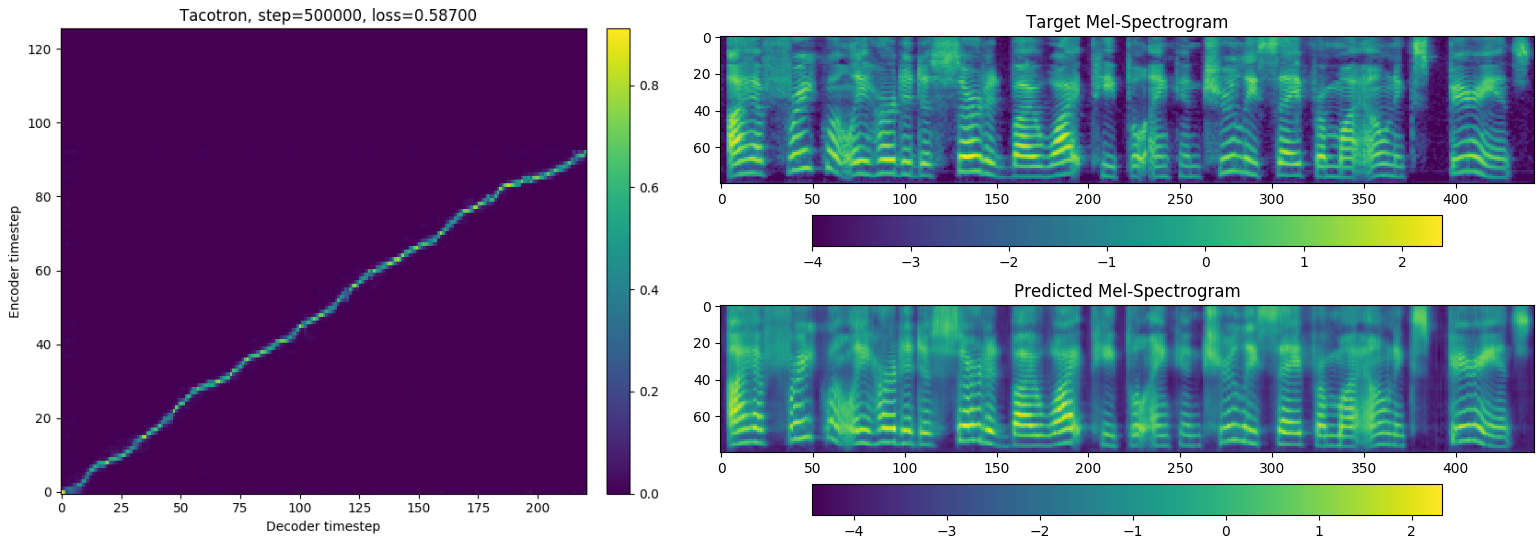
\includegraphics[width=\linewidth]{images/tacotron_alignment.png}
	\caption{(left) Example of alignment between the encoder steps and the decoder steps. (right) Comparison between the GTA predicted spectrogram and the ground truth spectrogram.}
	\label{tacotron_alignment}
\end{figure}

\color{red} griffin lim works but no characteristics, inference with punctuation? \color{black}


\subsection{Vocoder} \label{vocoder}
In SV2TTS and in Tacotron2, WaveNet is the vocoder. WaveNet has been at the heart of deep learning with audio since its release and remains state of the art when it comes to voice naturalness in TTS. It is however also known for being the slowest practical deep learning architecture at inference time. Several later papers brought improvements on that aspect to bring the generation near real-time or faster than real-time, e.g. \citep{ParallelWaveNet, FastWaveNet, WaveRNN}, with no or next to no hit to the quality of the generated speech. Nonetheless, WaveNet remains the vocoder in SV2TTS as speed is not the main concern in \citep{SV2TTS} and because Google's own WaveNet implementation with various improvements already generates at 8000 samples per second \citep[page~2]{WaveRNN}. This is in contrast with "vanilla" WaveNet which generates 172 steps per second at best \citep[page 7]{ParallelWaveNet}. At the time of the writing of this thesis, most open-source implementations of WaveNet are still vanilla implementations.

\citep{WaveRNN} proposes a simple scheme for describing the inference speed of autoregressive models. Given a target vector $\mathbf{u}$ with $|\mathbf{u}|$ samples to predict, the total time of inference $T(\mathbf{u})$ can be decomposed as:
$$ T(\mathbf{u}) = |\mathbf{u}|\sum_{i=1}^{N}(c(op_i) + d(op_i)) $$
where $N$ is the number of matrix-vector products ($\propto$ the number of layers) required to produce one sample, $c(op_i)$ is the computation time of layer $i$ and $d(op_i)$ is the overhead of the computation (typically I/O operations) for layer $i$. Note that standard sampling rates for speech include 16kHz, 22.05kHz and 24kHz (while music is usually sampled at 44.1kHz), meaning that for just 5 seconds of audio $|\mathbf{u}|$ is close to 100,000 samples. The standard WaveNet architecture accounts for three stacks of 10 residual blocks of two layers each, leading to $N = 60$. 

WaveRNN, the model proposed in \citep{WaveRNN}, improves on WaveNet by not only reducing the contribution from $N$ but also from $\mathbf{u}$, $c(op_i)$ and $d(op_i)$. The vocoder model we use is an open source implementation\footnote{\url{https://github.com/fatchord/WaveRNN}} that is based on WaveRNN but presents quite a few different design choices made by github user fatchord. We'll refer to this architecture as the "alternative WaveRNN".

\subsubsection{Model architecture}
In WaveRNN, the entire 60 convolutions from WaveNet are replaced by a single GRU layer \citep{GRU}. The authors maintain that the high non-linearity of a GRU layer alone is close enough to encompass the complexity of the entire WaveNet model. Indeed, they report a MOS of $4.51 \pm 0.08$ for Wavenet and $4.48 \pm 0.07$ for their best WaveRNN model. The forward pass of WaveRNN is implemented with only $N = 5$ matrix-vector products in a coarse-fine scheme where the lower 8 bits (coarse) of the target 16 bits sample are predicted first and then used to condition the prediction of the higher 8 bits (fine). The prediction is over the parameters of a distribution from which the output is sampled. We refer the reader to \citep{WaveRNN} for additional details.

The authors improve on the factors $c(op_i)$ and $d(op_i)$ by implementing the sampling operation as a custom GPU operation. We do not replicate this. They also sparsify the network with the pruning strategy from \citep{SparsityRNN, 2PruneOrNot2Prune}. This method gradually prunes weights during training, as opposed to more classical pruning algorithms that operate between several trainings. The algorithm creates a binary mask over the weights that indicates whether the weight should be forced set to 0 or remain as is. The proportion of zero weights compared to the total number of weights in the network is called sparsity. Results from \citep{SparsityRNN, 2PruneOrNot2Prune} indicate that large networks with sparsity levels between 90 and 95\% significantly outperform their dense versions. The authors of WaveRNN additionally argue that $c(op_i)$ is proportional to the number of nonzero weights. We experiment with this form of pruning and report our results in section \rw.

Finally, they propose 




\color{red} sparsity speed tests \color{black}

\clearpage
\bibliographystyle{plainnat}
\bibliography{references} 




















%$$\Leftrightarrow h_b(x) =
%\left\{\begin{array}{lll}
%0 & if & P(y = 0 | x) > P(y = 1 | x)\\ 
%1 & else &
%\end{array}\right.$$



%\begin{figure}[h]
%	\centering
%	\includegraphics[width=16cm]{image.png}
%	\caption{caption}
%	\label{label}
%\end{figure}



%\begin{figure}[h]
%	\centering
%	\captionsetup{justification=centering}
%	\hspace{-1cm}
%	\subfigure{\includegraphics[height=5cm]{image.png}}
%	\subfigure{\includegraphics[height=5cm]{image.png}}
%	\hspace{-1cm}
%	\caption{caption}
%	\label{label}
%\end{figure}


%\begin{center}
%	\begin{tabular}{|r|ccc|ccc|}
%		\hline
%		& \multicolumn{6}{c|}{Validation set}\\
%		\hline
%		& \multicolumn{3}{c|}{Valid images (3126)} & \multicolumn{3}{c|}{Invalid images (3126)} \\
%		\hline
%		& Correct & Unclassified & Incorrect & Correct & Unclassified & Incorrect \\
%		\hline
%		Reduced & 94.98\% & 3.07\% & 1.95\% & 95.27\% & 2.91\% & 1.82\% \\
%		Lenet & 98.08\% & 0.74\% & 1.18\% & 97.86\% & 0.96\% & 1.18\% \\
%		\hline
%	\end{tabular}
%	
%	\vspace{0.5cm}
%	  
%	\begin{tabular}{|r|ccc|ccc|}
%		\hline
%		& \multicolumn{6}{c|}{Test set}\\
%		\hline
%		& \multicolumn{3}{c|}{Valid images (999)} & \multicolumn{3}{c|}{Invalid images (74)} \\
%		\hline
%		& Correct & Unclassified & Incorrect & Correct & Unclassified & Incorrect \\
%		\hline
%		Reduced& 94.29\% & 3.70\% & 2.00\% & 95.95\% & 4.05\% & 0.00\%  \\
%		Lenet & 96.90\% & 1.30\% & 1.80\% & 97.30\% & 1.35\% & 1.35\% \\
%		\hline
%	\end{tabular}
%\end{center}


\end{document}













































































































